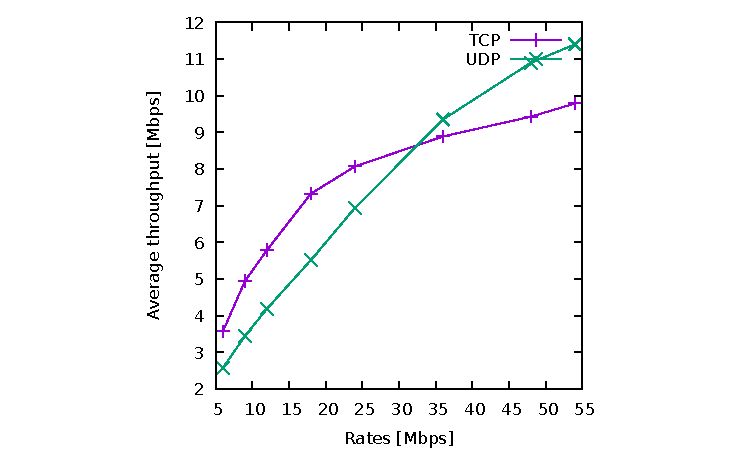
\includegraphics[width=0.5\textwidth]{traces/L3-2-1-tput.pdf}
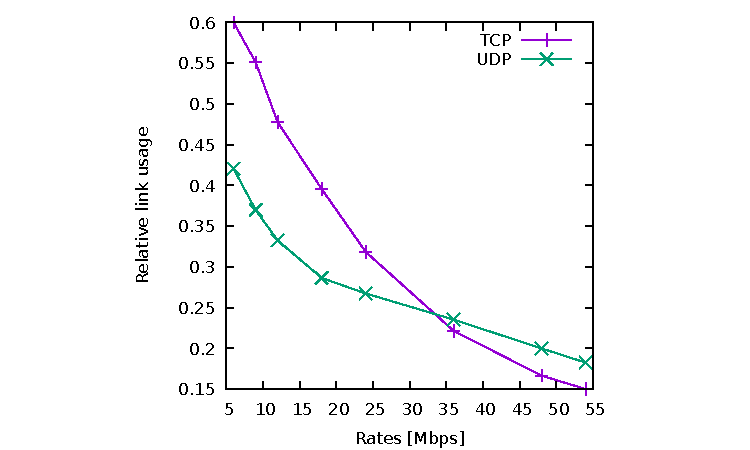
\includegraphics[width=0.5\textwidth]{traces/L3-2-1-usage.pdf}
For low bitrates TCP performs better than UDP. Due to TCP's congestion control there are fewer collisions compared to UDP. With lower bitrates the attainable maximum throughput is lower. This means TCP's slow start will reach it faster. The shorter the slow start phase, the smaller its negative effect on throughput can be. For lower bitrates this makes TCP perform better than UDP. For higher bitrates the influence of TCP's additional overhead and negative effect of congestion control become larger and UDP is more performant than TCP again. \\ \\
For both TCP and UDP, throughput in this case is roughly half of the previous test. Each packet is transmitted twice (to the AP and from the AP), halving the total throughput between source and destination. \\ \\
 The effect of increasing bitrate on the usage is similar to the previous test.
